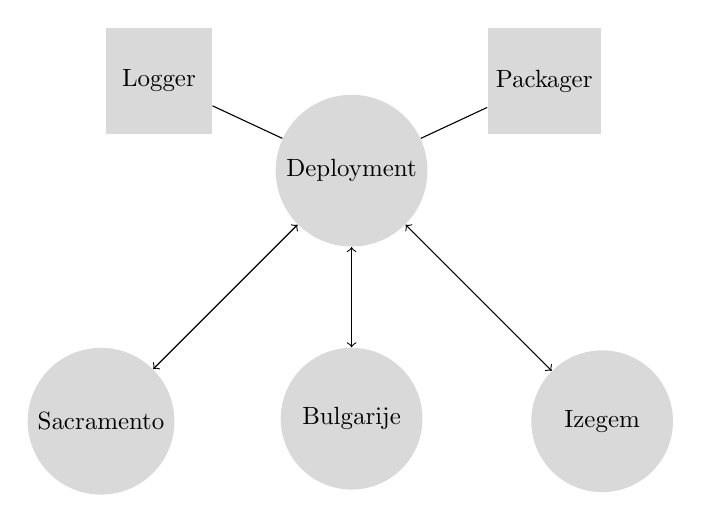
\begin{tikzpicture}[scale=.9, transform shape]
\tikzstyle{every node} = [circle, minimum size = 2cm, fill=gray!30]
\node (a) at (0, 0) {Deployment};
\node[shape = rectangle,minimum size = 1.5cm] (packager) at +(25: 3) {Packager};
\node[shape = rectangle,minimum size = 1.5cm] (logger) at +(155: 3) {Logger};
\node (b) at +(225: 5) {Sacramento};
\node (c) at +(270: 3.5) {Bulgarije};
\node (d) at +(315: 5) {Izegem};
\foreach \from/\to in {a/b, a/c, a/d}
\draw [<->] (\from) -- (\to);
\draw [-] (a) -- (packager);
\draw [-] (a) -- (logger);
\end{tikzpicture}